\section{Distributed crawling(splitting by key range vs. hash of key)}
\begin{figure}[h!]
  \centering
  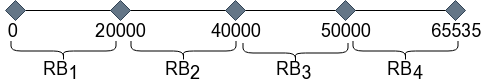
\includegraphics[width=10cm,height=4cm,keepaspectratio]{../media/crawler/requestboundaries.png}
  \caption{partitioning by hash of key}
  \label{fig:requestboundary}
\end{figure}

\begin{figure}[h!]
  \centering
  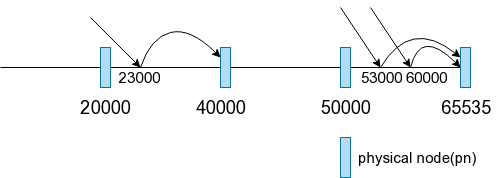
\includegraphics[width=10cm,height=4cm,keepaspectratio]{../media/crawler/modnsplit.png}
  \caption{Rebalancing physical nodes by mod N}
  \label{fig:modnsplit}
\end{figure}

\begin{figure}[h!]
  \centering
  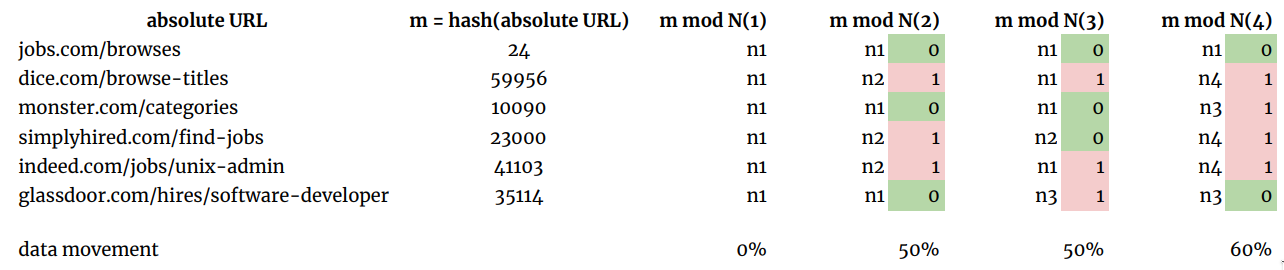
\includegraphics[width=16cm,height=8cm,keepaspectratio]{../media/crawler/modn_info.png}
  \caption{data movement when using modulo N}
  \label{fig:movemodn}
\end{figure}

\begin{figure}[h!]
  \centering
  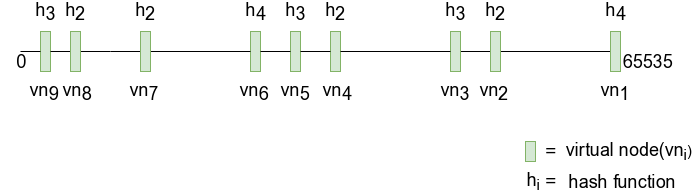
\includegraphics[width=12cm,height=5cm,keepaspectratio]{../media/crawler/vnodesplit1.png}
  \caption{virtual nodes to reduce shifts in data movements between nodes}
  \label{fig:vnodesplit1}
\end{figure}

\begin{figure}[h!]
  \centering
  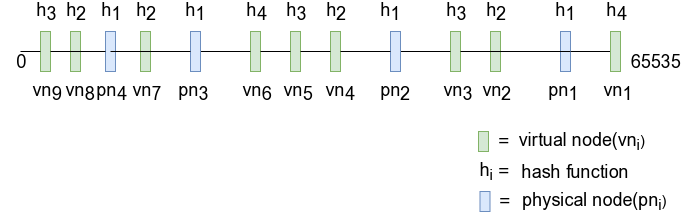
\includegraphics[width=12cm,height=5cm,keepaspectratio]{../media/crawler/vnodesplit2.png}
  \caption{Rebalancing physical nodes with virtual nodes}
  \label{fig:vnodesplit2}
\end{figure}

\begin{figure}[h!]
  \centering
  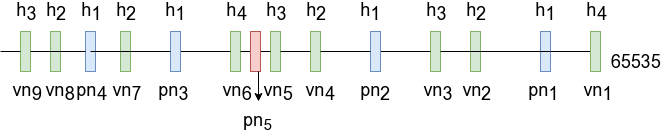
\includegraphics[width=12cm,height=5cm,keepaspectratio]{../media/crawler/addingnode.png}
  \caption{adding new node to existing cluster of nodes}
  \label{fig:addingnode}
\end{figure}

\begin{figure}[h!]
  \centering
  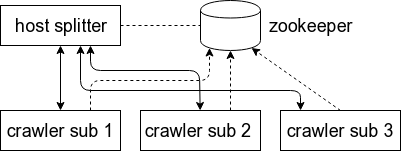
\includegraphics[width=8cm,height=5cm,keepaspectratio]{../media/crawler/zookeeper.png}
  \caption{zookeeper used to maintain up-to-date information on which vnodes are assigned to pnodes}
  \label{fig:zookeeper}
\end{figure}

\begin{figure}[h!]
  \centering
  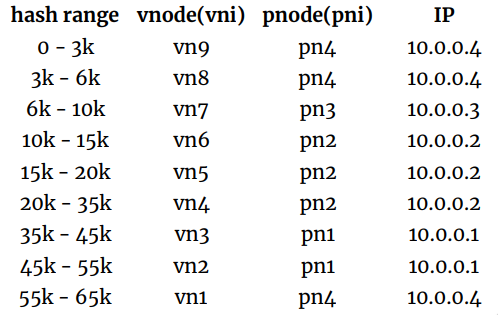
\includegraphics[width=8cm,height=5cm,keepaspectratio]{../media/crawler/zookeeper_info.png}
  \caption{zookeeper table}
  \label{fig:zookeeper_info}
\end{figure}

\pagebreak
